\section{Ellen (O'Brien) Duggan}\label{per:Ellen3OBrien}

\index{O'Brien!Ellen\textsuperscript{3} (1857--1927)|bb}\index{Duggan!Ellen\textsuperscript{3} (O'Brien)|bb} 
\MainPerson{Ellen\textsuperscript{3} O'Brien} (\Lineage{2}{Michael}, \Lineage{1}{William}) was born in Boston, Suffolk County, Massachusetts, probably on 16 July 1857.\cite{Ellen3OBrien3Birth} She was likely\footnote{This baptismal record lists parents as Michael O'Brien and Bridget Colman, which could be a misspelling of Colbert. The 1870 census, the first definitive record of Ellen, places her birth between 8 July 1857 and 7 July 1858.} baptized at St.\ John the Baptist Church in Boston (North End) on 18 July 1857.\cite{Ellen3OBrien3Baptism} She died in Lynn, Essex County, Massachusetts, on 29 July 1927 and was buried at Holy Cross Cemetery in Malden, Middlesex County, Massachusetts.\cite{Ellen3OBrien3Death} Ellen married, at Most Holy Redeemer Church in East Boston on 14 January 1891, \MainPerson{Patrick J.\ Duggan} (aka Durgan).\cite{Ellen3OBrien3Marriage:1}\index{Duggan!Patrick J.|bb}\index{Durgan!Patrick J.|see {Duggan!Patrick J.}} Patrick was born in Ireland on February 1862\cite{Census1900Ellen3OBrien3} to James Durgan and Catharine (\_\_\_\_\_) Durgin.\cite{Ellen3OBrien3Marriage:2} He died in East Boston on 6 April 1922 and was buried with Ellen at Holy Cross Cemetery.\cite{PatrickDugganDeath}

In 1880, Ellen was living with her father and stepmother in East Boston and working at a store.\cite{Census1880Ellen3OBrien3} She married Patrick Duggan, who immigrated from Ireland in 1882. He was working as a longshoreman in 1900.\cite{Census1900Ellen3OBrien3} In 1910, Patrick was working as a laborer at a lumber yard, Ellen was a cleaner at an office building, and son William was an apprentice at a shoe factory.\cite{Census1910Ellen3OBrien3} In 1920, Patrick and son Edward were both working as teamsters at trucking companies, while Mary was a telephone operator.\cite{Census1920Ellen3OBrien3}

\begin{KidsIntro}
	Children of Patrick J.\ Duggan and Ellen\textsuperscript{3} (O'Brien) Duggan:
\end{KidsIntro}

\begin{Kids}
	
\KidNum{}{i.}\KidName{Esther Catharine\textsuperscript{4}  Duggan},\index{Duggan!Esther Catharine\textsuperscript{4}} b.\ Boston, 29 March 1891;\cite{EstherDugganBirth} bap.\ Sacred Heart, Boston, 5 April 1891;\cite{EstherDugganBaptism} d.\ Boston, 30 March 1892 (hydrocephalus);\cite{EstherDugganDeath} bur.\ Catholic Mt.\ Auburn Cemetery, Watertown, Middlesex, Mass.\cite{EstherDugganBurial}

\KidNum{}{ii.}\KidName{William James Duggan}\index{Duggan!William\textsuperscript{4} James}, b.\ Boston, 5 Oct.\ 1892;\cite{WilliamDugganBirth} bap.\ Sacred Heart, East Boston, 16 Oct.\ 1892;\cite{WilliamDugganBaptism} d.\ Chelsea Soldiers' Home, Chelsea, Suffolk County, Mass., 23 Sept.\ 1970. William was a cook by trade.\cite{WilliamDugganDeath:1} He served in the Navy during WWI and in the U.S.\ Lighthouse Service (which later merged with the Coast Guard\cite{Lighthouse}) after the war.\cite{protection} During WWII he likely served in the Army National Guard, Medical Department.\cite{WilliamDugganWWII}

\KidNum{}{iii.}\KidName{Mary Frances Duggan}\index{Duggan!Mary Frances\textsuperscript{4}}\index{Johnson!Mary Frances\textsuperscript{4}}\index{MacLean!Mary Frances\textsuperscript{4}}

\KidNum{\ref{per:Edward4Duggan}}{iv.}\KidName{Edward Joseph Duggan}\index{Duggan!Edward Joseph\textsuperscript{4}}, b.\ Boston, 28 Dec.\ 1898; m.\ Boston, 19 Aug.\ 1920, \KidName{Anna M.\ Spracklin}.

\begin{figure}[htbp]
	\centering
	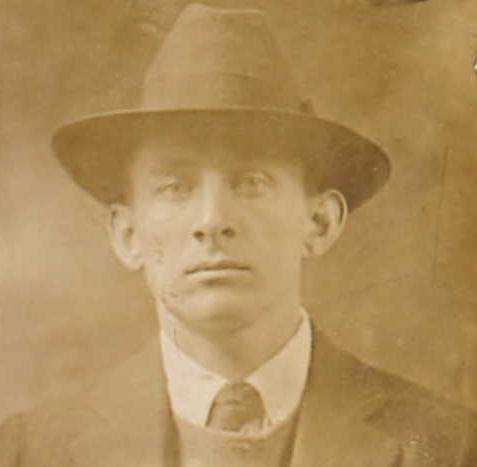
\includegraphics[width=1.59in]{William_J_Duggan}
	\caption{William J.\ Duggan's photograph attached to his application for a Seaman's Protection Certificate in 1919.}
	\label{fig:WilliamDuggan}
\end{figure}

\end{Kids}